\documentclass[a4paper]{article}

\def\npart {III}
\def\nterm {Easter}
\def\nyear {2017}
\def\nlecturer {N.\ S.\ Manton}
\def\ncourse {Classical and Quantum Solitons}

% Imports
\ifx \nextra \undefined
  \usepackage[pdftex,
    hidelinks,
    pdfauthor={Dexter Chua},
    pdfsubject={Cambridge Maths Notes: Part \npart\ - \ncourse},
    pdftitle={Part \npart\ - \ncourse},
  pdfkeywords={Cambridge Mathematics Maths Math \npart\ \nterm\ \nyear\ \ncourse}]{hyperref}
  \title{Part \npart\ - \ncourse}
\else
  \usepackage[pdftex,
    hidelinks,
    pdfauthor={Dexter Chua},
    pdfsubject={Cambridge Maths Notes: Part \npart\ - \ncourse\ (\nextra)},
    pdftitle={Part \npart\ - \ncourse\ (\nextra)},
  pdfkeywords={Cambridge Mathematics Maths Math \npart\ \nterm\ \nyear\ \ncourse\ \nextra}]{hyperref}

  \title{Part \npart\ - \ncourse \\ {\Large \nextra}}
\fi

\author{Lectured by \nlecturer \\\small Notes taken by Dexter Chua}
\date{\nterm\ \nyear}

\usepackage{alltt}
\usepackage{amsfonts}
\usepackage{amsmath}
\usepackage{amssymb}
\usepackage{amsthm}
\usepackage{booktabs}
\usepackage{caption}
\usepackage{enumitem}
\usepackage{fancyhdr}
\usepackage{graphicx}
\usepackage{mathtools}
\usepackage{microtype}
\usepackage{multirow}
\usepackage{pdflscape}
\usepackage{pgfplots}
\usepackage{siunitx}
\usepackage{tabularx}
\usepackage{tikz}
\usepackage{tkz-euclide}
\usepackage[normalem]{ulem}
\usepackage[all]{xy}

\pgfplotsset{compat=1.12}

\pagestyle{fancyplain}
\lhead{\emph{\nouppercase{\leftmark}}}
\ifx \nextra \undefined
  \rhead{
    \ifnum\thepage=1
    \else
      \npart\ \ncourse
    \fi}
\else
  \rhead{
    \ifnum\thepage=1
    \else
      \npart\ \ncourse\ (\nextra)
    \fi}
\fi
\usetikzlibrary{arrows}
\usetikzlibrary{decorations.markings}
\usetikzlibrary{decorations.pathmorphing}
\usetikzlibrary{positioning}
\usetikzlibrary{fadings}
\usetikzlibrary{intersections}
\usetikzlibrary{cd}

\newcommand*{\Cdot}{\raisebox{-0.25ex}{\scalebox{1.5}{$\cdot$}}}
\newcommand {\pd}[2][ ]{
  \ifx #1 { }
    \frac{\partial}{\partial #2}
  \else
    \frac{\partial^{#1}}{\partial #2^{#1}}
  \fi
}

% Theorems
\theoremstyle{definition}
\newtheorem*{aim}{Aim}
\newtheorem*{axiom}{Axiom}
\newtheorem*{claim}{Claim}
\newtheorem*{cor}{Corollary}
\newtheorem*{defi}{Definition}
\newtheorem*{eg}{Example}
\newtheorem*{fact}{Fact}
\newtheorem*{law}{Law}
\newtheorem*{lemma}{Lemma}
\newtheorem*{notation}{Notation}
\newtheorem*{prop}{Proposition}
\newtheorem*{thm}{Theorem}

\renewcommand{\labelitemi}{--}
\renewcommand{\labelitemii}{$\circ$}
\renewcommand{\labelenumi}{(\roman{*})}

\let\stdsection\section
\renewcommand\section{\newpage\stdsection}

% Strike through
\def\st{\bgroup \ULdepth=-.55ex \ULset}

% Maths symbols
\newcommand{\bra}{\langle}
\newcommand{\ket}{\rangle}

\newcommand{\N}{\mathbb{N}}
\newcommand{\Z}{\mathbb{Z}}
\newcommand{\Q}{\mathbb{Q}}
\renewcommand{\H}{\mathbb{H}}
\newcommand{\R}{\mathbb{R}}
\newcommand{\C}{\mathbb{C}}
\newcommand{\Prob}{\mathbb{P}}
\renewcommand{\P}{\mathbb{P}}
\newcommand{\E}{\mathbb{E}}
\newcommand{\F}{\mathbb{F}}
\newcommand{\cU}{\mathcal{U}}
\newcommand{\RP}{\mathbb{RP}}
\newcommand{\CP}{\mathbb{CP}}

\newcommand{\ph}{\,\cdot\,}

\DeclareMathOperator{\sech}{sech}
\DeclareMathOperator{\cosech}{cosech}
\DeclareMathOperator{\cosec}{cosec}

\DeclareMathOperator{\covol}{covol}
\DeclareMathOperator{\vol}{vol}

\let\Im\relax
\let\Re\relax
\DeclareMathOperator{\Im}{Im}
\DeclareMathOperator{\Re}{Re}
\DeclareMathOperator{\im}{im}
\DeclareMathOperator{\image}{image}
\DeclareMathOperator{\Ann}{Ann}

\DeclareMathOperator*{\res}{res}
\DeclareMathOperator{\Res}{Res}
\DeclareMathOperator{\Ind}{Ind}

\DeclareMathOperator{\tr}{tr}
\DeclareMathOperator{\diag}{diag}
\DeclareMathOperator{\rank}{rank}
\DeclareMathOperator{\card}{card}
\DeclareMathOperator{\spn}{span}
\DeclareMathOperator{\adj}{adj}

\DeclareMathOperator{\erf}{erf}
\DeclareMathOperator{\erfc}{erfc}

\DeclareMathOperator{\ord}{ord}
\DeclareMathOperator{\Sym}{Sym}

\DeclareMathOperator{\sgn}{sgn}
\DeclareMathOperator{\orb}{orb}
\DeclareMathOperator{\stab}{stab}
\DeclareMathOperator{\ccl}{ccl}

\DeclareMathOperator{\lcm}{lcm}
\DeclareMathOperator{\hcf}{hcf}

\DeclareMathOperator{\Int}{Int}
\DeclareMathOperator{\id}{id}

\DeclareMathOperator{\betaD}{beta}
\DeclareMathOperator{\gammaD}{gamma}
\DeclareMathOperator{\Poisson}{Poisson}
\DeclareMathOperator{\binomial}{binomial}
\DeclareMathOperator{\multinomial}{multinomial}
\DeclareMathOperator{\Bernoulli}{Bernoulli}
\DeclareMathOperator{\like}{like}

\DeclareMathOperator{\var}{var}
\DeclareMathOperator{\cov}{cov}
\DeclareMathOperator{\bias}{bias}
\DeclareMathOperator{\mse}{mse}
\DeclareMathOperator{\corr}{corr}

\DeclareMathOperator{\otp}{otp}
\DeclareMathOperator{\dom}{dom}

\DeclareMathOperator{\Root}{Root}
\DeclareMathOperator{\supp}{supp}
\DeclareMathOperator{\rel}{rel}
\DeclareMathOperator{\Hom}{Hom}
\DeclareMathOperator{\Aut}{Aut}
\DeclareMathOperator{\Gal}{Gal}
\DeclareMathOperator{\Mat}{Mat}
\DeclareMathOperator{\End}{End}
\DeclareMathOperator{\Char}{char}
\DeclareMathOperator{\ev}{ev}
\DeclareMathOperator{\St}{St}
\DeclareMathOperator{\Lk}{Lk}
\DeclareMathOperator{\disc}{disc}
\DeclareMathOperator{\Isom}{Isom}
\DeclareMathOperator{\length}{length}
\DeclareMathOperator{\energy}{energy}
\DeclareMathOperator{\area}{area}
\DeclareMathOperator{\Syl}{Syl}
\DeclareMathOperator{\cl}{cl}
\DeclareMathOperator{\fix}{fix}

\newcommand{\GL}{\mathrm{GL}}
\newcommand{\SL}{\mathrm{SL}}
\newcommand{\PGL}{\mathrm{PGL}}
\newcommand{\PSL}{\mathrm{PSL}}
\newcommand{\PSU}{\mathrm{PSU}}
\newcommand{\Or}{\mathrm{O}}
\newcommand{\SO}{\mathrm{SO}}
\newcommand{\U}{\mathrm{U}}
\newcommand{\SU}{\mathrm{SU}}

\renewcommand{\d}{\mathrm{d}}
\newcommand{\D}{\mathrm{D}}

\tikzset{->/.style = {decoration={markings,
                                  mark=at position 1 with {\arrow[scale=2]{latex'}}},
                      postaction={decorate}}}
\tikzset{<-/.style = {decoration={markings,
                                  mark=at position 0 with {\arrowreversed[scale=2]{latex'}}},
                      postaction={decorate}}}
\tikzset{<->/.style = {decoration={markings,
                                   mark=at position 0 with {\arrowreversed[scale=2]{latex'}},
                                   mark=at position 1 with {\arrow[scale=2]{latex'}}},
                       postaction={decorate}}}
\tikzset{->-/.style = {decoration={markings,
                                   mark=at position #1 with {\arrow[scale=2]{latex'}}},
                       postaction={decorate}}}
\tikzset{-<-/.style = {decoration={markings,
                                   mark=at position #1 with {\arrowreversed[scale=2]{latex'}}},
                       postaction={decorate}}}

\tikzset{circ/.style = {fill, circle, inner sep = 0, minimum size = 3}}
\tikzset{mstate/.style={circle, draw, blue, text=black, minimum width=0.7cm}}

\definecolor{mblue}{rgb}{0.2, 0.3, 0.8}
\definecolor{morange}{rgb}{1, 0.5, 0}
\definecolor{mgreen}{rgb}{0.1, 0.4, 0.2}
\definecolor{mred}{rgb}{0.5, 0, 0}

\def\drawcirculararc(#1,#2)(#3,#4)(#5,#6){%
    \pgfmathsetmacro\cA{(#1*#1+#2*#2-#3*#3-#4*#4)/2}%
    \pgfmathsetmacro\cB{(#1*#1+#2*#2-#5*#5-#6*#6)/2}%
    \pgfmathsetmacro\cy{(\cB*(#1-#3)-\cA*(#1-#5))/%
                        ((#2-#6)*(#1-#3)-(#2-#4)*(#1-#5))}%
    \pgfmathsetmacro\cx{(\cA-\cy*(#2-#4))/(#1-#3)}%
    \pgfmathsetmacro\cr{sqrt((#1-\cx)*(#1-\cx)+(#2-\cy)*(#2-\cy))}%
    \pgfmathsetmacro\cA{atan2(#2-\cy,#1-\cx)}%
    \pgfmathsetmacro\cB{atan2(#6-\cy,#5-\cx)}%
    \pgfmathparse{\cB<\cA}%
    \ifnum\pgfmathresult=1
        \pgfmathsetmacro\cB{\cB+360}%
    \fi
    \draw (#1,#2) arc (\cA:\cB:\cr);%
}
\newcommand\getCoord[3]{\newdimen{#1}\newdimen{#2}\pgfextractx{#1}{\pgfpointanchor{#3}{center}}\pgfextracty{#2}{\pgfpointanchor{#3}{center}}}

\def\Xint#1{\mathchoice
   {\XXint\displaystyle\textstyle{#1}}%
   {\XXint\textstyle\scriptstyle{#1}}%
   {\XXint\scriptstyle\scriptscriptstyle{#1}}%
   {\XXint\scriptscriptstyle\scriptscriptstyle{#1}}%
   \!\int}
\def\XXint#1#2#3{{\setbox0=\hbox{$#1{#2#3}{\int}$}
     \vcenter{\hbox{$#2#3$}}\kern-.5\wd0}}
\def\ddashint{\Xint=}
\def\dashint{\Xint-}


\usepackage[compat=1.1.0]{tikz-feynman}
\tikzfeynmanset{/tikzfeynman/momentum/arrow shorten = 0.3}
\tikzfeynmanset{/tikzfeynman/warn luatex = false}


\begin{document}
\maketitle
{\small
\setlength{\parindent}{0em}
\setlength{\parskip}{1em}
Solitons are solutions of classical field equations with particle-like properties. They are localised in space, have finite energy and are stable against decay into radiation. The stability usually has a topological explanation. After quantisation, they give rise to new particle states in the underlying quantum field theory that are not seen in perturbation theory. We will focus mainly on kink solitons in one space dimension, and on Skyrmions in three dimensions. Solitons in gauge theories will also be mentioned.

\subsubsection*{Pre-requisites}
This course assumes you have taken Quantum Field Theory and Symmetries, Fields and Particles. The small amount of topology that is needed will be developed during the course.
}
\tableofcontents

\setcounter{section}{-1}
\section{Introduction}
Given a classical field theory, if we want to ``quantize'' it, then we find the vacuum of the theory, and then do perturbation theory around this vacuum. If there are multiple vacua, then what we did was that we arbitrarily picked a vacuum, and then expanded around that vacuum.

However, these field theories with multiple vacua often contain \emph{soliton} solutions. These are localized, smooth solutions of the classical field equations, and they ``connect multiple vacuums''. To quantize these solitons solutions, we fix such a soliton, and use it as the ``background''. We then do perturbation theory around these solutions, but this is rather tricky to do. Thus, in a lot of the course, we will just look at the classical part of the theory.

Recall that when quantizing our field theories in perturbation theory, we obtain particles in the quantum theory, despite the classical theory being completely about fields. It turns our solitons also behave like particles, and they are a \emph{new} type of particles. These are non-perturbative phenomenon. If we want to do the quantum field theory properly, we have to include these solitons in the quantum field theory. In general this is hard, and so we are not going to develop this a lot.

What does it mean to say that solitons are like particles? In relativistic field theories, we find these solitons have a classical energy. We define the ``mass'' $M$ of the soliton to be the energy in the ``rest frame''. Since this is relativistic, we can do a Lorentz boost, and we obtain a moving soliton. Then we obtain a relation of the form
\[
  E^2 - \mathbf{P} \cdot \mathbf{P} = M^2.
\]
This is a Lorentz-invariant property of the soliton. Together with the fact that the soliton is localized, this is a justification for thinking of them as particles.

These particles differ from the particles perturbative quantum fields, as they have rather different properties. Interesting solitons have a \emph{topological} character different from the classical vacuum. Thus, at least naively, they cannot be thought of perturbatively.

There are also non-relativistic solitons, and they usually don't have interpretations of particles. These appear, for example, as defects in solids. We will not be interested in these much.

What kinds of theories have solitons? To obtain solitons, we definitely need a non-linear field structure and/or non-linear equations. Thus, free field theories with quadratic Lagrangians such as Maxwell theory do not have solitons. We need interaction terms.

Note that in QFT, we did interactions using the interaction picture. We split the Hamiltonian into a ``free field'' part, which we solve exactly, and the ``interaction'' part. However, to quantize solitons, we need to solve the full interacting Lagrangian \emph{exactly}.

Having interactions is not enough for solitons to appear. To obtain solitons, we also need some non-trivial vacuum topology. In other words, we need more than one vacuum. This usually comes from symmetry breaking, and often gauge symmetries are involved.

In this course, we will focus on three types of solitons.
\begin{itemize}
  \item In one (space) dimension, we have kinks. We will spend $4$ lectures on this.

  \item In two dimensions, we have vortices. We will spend $6$ lectures on this.

  \item In three dimensions, there are monopoles and Skyrmions. We will only study Skyrmions, and will spend $6$ lectures on it.
\end{itemize}
These examples are all relativistic. Non-relativistic solitons include \emph{domain walls}, which occur in ferromagnets, but we will not study these.

In general, solitons appear in all sorts of different actual, physical scenarios such as in condensed matter physics, optical fibers, superconductors, ``cosmic strings'' etc. Since we are mathematicians, we probably will not put much focus on these actual applications. However, we can talk a bit more about Skyrmions.

Skyrmions are solitons in an \emph{effective field theory} of interacting pions, which are thought to be the most important baryons because they are the lightest. This happens in spite of the lack of a gauge symmetry. While pions have no baryon number, the associated solitons have a topological charge identified with baryon number. This baryon number is conserved for topological reasons.

Note that in QCD, baryon number is conserved because the quark number is conserved. We tried extremely hard to find proton decay, which would be a process that involves baryon numbers, but we cannot find such examples. We have very high experimental certainty that baryon number is conserved. And if baryon number is topological, then this is a very good reason for the conservation of baryon numbers.

Skyrmions give a model of low-energy interactions of baryons. This leads to an (approximate) theory of nucleons (proton and neutron) and larger nuclei, which are bound states of any number of protons and neutrons. % This is really up-to-date stuff.

There is a whole other set of Skyrmions studied, which are two-dimensional. These are structure in exotic magnets, and they have actually been seen.

For these ideas to work out well, we need to eventually do quantization. For example, Skyrmions by themselves do not have spin. We need to quantize the theory before these come out. Also, Skyrmions cannot distinguish between protons and neutrons. These differences only come up after we quantize.
\section{\tph{$\phi^4$}{phi4}{&straightphi;<sup>4</sup>} kinks}
\subsection{Kink solutions}
In this chapter, we are going to study \term{$\phi^4$ kinks}\index{kink}\index{kink!$\phi^4$}. This happens in $1 + 1$ dimensions, and involves a single scalar field $\phi(x, t)$. In higher dimensions, we often need many fields to obtain solitons, but in the case of 1 dimension, we can get away with a single field.

In general, the \term{Lagrangian density} of such a scalar field theory is of the form
\[
  \mathcal{L} = \frac{1}{2} \partial_\mu \phi \partial^\mu \phi - U(\phi)
\]
for some potential $U(\phi)$ polynomial in $\phi$. Note that in $1 + 1$ dimensions, any such theory is renormalizable. Here we will choose the Minkowski metric to be
\[
  \eta^{\mu\nu} =
  \begin{pmatrix}
    1 & 0\\
    0 & -1
  \end{pmatrix}.
\]
Then the \term{Lagrangian} is given by
\[
  L = \int_{-\infty}^\infty \mathcal{L}\;\d x = \int_{-\infty}^\infty \left(\frac{1}{2} \partial_\mu \phi \partial^\mu \phi - U(\phi)\right)\;\d x,
\]
and then the \term{action} is
\[
  S[\phi] = \int L\;\d t = \int \mathcal{L} \;\d x\;\d t.
\]

There is a non-linearity in the field equations due to a potential $U(\phi)$ with \emph{multiple vacua}. We need this multiple vacua to obtain a soliton. The kink stability comes from the \emph{topology}. It is very simple here, and just comes from counting the discrete, distinct vacua.

As usual, we will write
\[
  \dot{\phi} = \frac{\partial \phi}{\partial t},\quad \phi' = \frac{\partial \phi}{\partial x}.
\]
Often it is convenient to (non-relativistically) split the Lagrangian as
\[
  L = T - V,
\]
where
\[
  T = \int \frac{1}{2} \dot{\phi}^2\;\d x,\quad V = \int \left(\frac{1}{2} \phi'^2 + U(\phi)\right)\;\d x.
\]
In higher dimensions, we separate out $\partial_\mu \phi$ into $\dot{\phi}$ and $\nabla \phi$.

The classical field equation comes from the condition that $S[\phi]$ is stationary under variations of $\phi$. By a standard manipulation, the field equation turns out to be
\[
  \partial_\mu \partial^\mu \phi + \frac{\d U}{\d \phi} = 0.
\]
This is an example of a Klein--Gordon type of field equation, but is non-linear if $U$ is not quadratic. This is known as the \term{non-linear Klein--Gordon equation}\index{Klein--Gordon equation!non-linear}.

We are interested in a soliton that is a static solution. For a static field, the time derivatives can be dropped, and this equation becomes
\[
  \frac{\d^2 \phi}{\partial x^2} = \frac{\d U}{\d \phi}.
\]
Of course, the important part is the choice of $U$! In $\phi^4$ theory, we choose
\[
  U(\phi) = \frac{1}{2} (1 - \phi^2)^2.
\]
This is mathematically the simplest version, because we set all coupling constants to $1$. If we want to quantize this (or just want to be more sophisticated), then we should include some parameters. However, this tends to become a complete mess.

The importance of this $U$ is that it has two minima:
\begin{center}
  \begin{tikzpicture}
    \draw [->](-3, -1) -- (3, -1) node [right] {$\phi$};
    \draw [->] (0, -1.5) -- (0, 3) node [above] {$U(\phi)$};

    \draw [mblue, thick, domain=-2.4:2.4, samples=50] plot [smooth] (\x, {4 * ((\x/2)^4 - (\x/2)^2)});

    \node at (-1.414, -1) [below] {$-1$};
    \node at (1.414, -1) [below] {$1$};
  \end{tikzpicture}
\end{center}
The two classical vacuum are
\[
  \phi(x) \equiv 1,\quad \phi(x) \equiv -1.
\]
This is, of course, not the only possible choice. We can, for example, include some parameters and set
\[
  U(\phi) = \lambda(m^2 - \phi^2)^2.
\]
If we are more adventurous, we can talk about a $\phi^6$ theory with
\[
  U(\phi) = \lambda \phi^2 (m^2 - \phi^2)^2.
\]
In this case, we have $3$ minima, instead of $2$. Even braver people can choose
\[
  U(\phi) = 1 - \cos \phi.
\]
This has \emph{infinitely} many minima. The field equation involves a $\sin \phi$ term, and is hence this theory is called the \term{sine-Gordon theory} (a pun on the name Klein--Gordon, of course).

The sine-Gordon theory is a special case. While it seems like the most complicated potential so far, it is actually \term{integrable}. This implies we can find explicit exact solutions involving multiple, interacting solitons in a rather easy way. However, integrable systems is a topic for another course, namely the IID Integrable Systems course.

For now, we will focus on our simplistic $\phi^4$ theory. As mentioned, there are two vacuum field configurations, both of zero energy. We will in general use the term ``\term{field configuration}'' to refer to fields that are not necessarily solutions to the classical field equation, but in this case, the vacua are indeed solutions.

If we wanted to quantize this $\phi^4$ theory, then we have to pick one of the vacua and do perturbation theory around it. This is known as \term{spontaneous symmetry breaking}. Of course, by symmetry, we obtain the same quantum theory regardless of which vacuum we expand around.

However, as we mentioned, when we want to study solitons, we have to involve \emph{both} vacua. We want to consider solutions that ``connect'' these two vacua. In other words, we are looking for solutions that look like
\begin{center}
  \begin{tikzpicture}
    \draw [->] (-3, 0) -- (3, 0) node [right] {$x$};
    \draw [->] (0, -2) -- (0, 2) node [above] {$m$};

    \draw [mblue, thick, domain=-3:3] plot [smooth] (\x, {tanh(1.5*(\x + 1))});

    \draw [dashed] (-3, 1) -- (3, 1);
    \draw [dashed] (-3, -1) -- (3, -1);

    \node [circ] at (-1, 0) {};
    \node [anchor = north west] at (-1, 0) {$a$};
  \end{tikzpicture}
\end{center}
This is known as a \term{kink solution}.

To actually find such a solution, we need the full field equation, given by
\[
  \frac{\d^2 \phi}{\d x^2} = -2 (1 - \phi^2) \phi.
\]
Instead of solving this directly, we will find the kink solutions by considering the energy, since this method generalizes better.

We will work with a general potential $U$ with minimum $0$. From Noether's theorem, we obtain a conserved energy
\[
  E = \int \left(\frac{1}{2} \dot{\phi}^2 + \frac{1}{2} \phi'^2 + U(\phi)\right)\;\d x.
\]
For a static field, we drop the $\dot{\phi}^2$ term. Then this is just the $V$ appearing in the Lagrangian. By definition, the field equation tells us the field is a stationary point of this energy. To find the kink solution, we will in fact find a \emph{minimum} of the energy.

Of course, the global minimum is attained when we have a vacuum field, in which case $E = 0$. However, this is just the global minimum only if we don't impose any boundary conditions. In our case, the kinks satisfy the boundary conditions ``$\phi(\infty) = 1$'', ``$\phi(-\infty) = -1$'' (interpreted in terms of limits, of course). The kinks will minimize energy subject to these boundary conditions.

These boundary conditions are important, because they are ``topological''. Eventually, we will want to understand the dynamics of solitons, so we will want to consider fields that evolve with time. From physical considerations, for any fixed $t$, the field $\phi(x, t)$ must satisfy $\phi(x, t) \to \text{vacuum}$ as $x \to \pm \infty$, or else the field will have infinite energy. However, the vacuum of our potential $U$ is discrete. Thus, if $\phi$ were to evolve continuously with time, the boundary conditions must not evolve with time! At least, this is what we expect classically. Who knows what weird tunnelling can happen in quantum field theory.

So from now on, we fix a some boundary conditions $\phi(\infty)$ and $\phi(-\infty)$, and focus on fields that satisfy these boundary conditions. The trick is to write the potential in the form
\[
  U (\phi) = \frac{1}{2} \left(\frac{\d W (\phi)}{\d \phi}\right)^2.
\]
If $U$ is always non-negative, then we can always find $W$ in principle --- we take the square root and then integrate it. However, in practice, this is useful only if we can find a simple form for $W$. Let's assume we've done that. Then we can write
\begin{align*}
  E &= \frac{1}{2} \int \left(\phi'^2 + \left(\frac{\d W}{\d \phi}\right)^2 \right)\;\d x\\
  &= \frac{1}{2} \int \left(\phi' \mp \frac{\d W}{\d \phi}\right)^2\;\d x \pm \int \frac{\d W}{\d \phi} \frac{\d \phi}{\d x} \;\d x\\
  &= \frac{1}{2} \int \left(\phi' \mp \frac{\d W}{\d \phi}\right)^2\;\d x \pm \int \d W\\
  &= \frac{1}{2} \int \left(\phi' \mp \frac{\d W}{\d \phi}\right)^2\;\d x \pm (W(\phi(\infty)) - W(\phi(-\infty))).
\end{align*}
The second term depends purely on the boundary conditions, which we have fixed. Thus, we can minimize energy if we can make the first term vanish! Note that when completing the square, the choice of the signs is arbitrary. However, if we want to set the first term to be $0$, the second term had better be non-positive, since the energy itself is non-negative! Hence, we will pick the sign such that the second term is $\geq 0$, and then the energy is minimized when
\[
  \phi' = \pm \frac{\d W}{\d \phi}.
\]
In this case, we have
\[
  E = \pm (W(\infty) - W(-\infty)).
\]
These are known as the \term{Bogomolny equation} and the \term{Bogomolny energy bound}. Note that if we picked the other sign, then we cannot solve the differential equation $\phi' = \pm \frac{\d W}{\d \phi}$, because we know the energy must be non-negative.

For the $\phi^4$ kink, we have
\[
  \frac{\d W}{\d \phi} = 1 - \phi^2.
\]
So we pick
\[
  W = \phi - \frac{1}{3} \phi^3.
\]
So when $W = \pm 1$, we have $W = \pm \frac{2}{3}$. We need to choose the $+$ sign, and then we know the energy (and hence mass) of the kink is
\[
  E \equiv M = \frac{4}{3}.
\]
We now solve for $\phi$. The equation we have is
\[
  \phi' = 1 - \phi^2.
\]
Rearranging gives
\[
  \frac{1}{1 - \phi^2} \d \phi = \d x,
\]
which we can integrate to give
\[
  \phi (x) = \tanh (x - a).
\]
This $a$ is an arbitrary constant of integration, labelling the intersection with the $x$-axis. We think of this as the ``\term{location}'' of the kink.

Note that there is not a unique solution, which is not unexpected by translation invariance. Instead, the solutions are labeled by a parameter $a$. This is known as a \term{modulus} of the solution. In general, there can be multiple moduli, and the space of all possible values of the moduli is known as the \term{moduli space}. In this case, the moduli space is just $\R$.

Is this solution stable? We obtained this kink solution by minimizing the energy within this topological class of solutions (i.e.\ among all solutions with the prescribed boundary conditions). Since a field cannot change the boundary conditions during evolution, it follows that the kink must be stable.

Are there other soliton solutions to the field equations? The solutions are determined by the boundary conditions. Thus, we can classify all soliton solutions by counting all possible combinations of the boundary conditions. We have, of course, two vacuum solutions $\phi \equiv 1$ and $\phi \equiv -1$. There is also an \term{anti-kink}\index{kink!anti-} solution obtained by inverting the kink:
\[
  \phi(x) = - \tanh (x - b).
\]
This also has energy $\frac{4}{3}$.

\subsection{Dynamic kink}
We now want to look at kinks that move. Given what we have done so far, this is trivial. Our theory is Lorentz invariant, so we simply apply a Lorentz boost. Then we obtain a field
\[
  \phi(x, t) = \tanh \gamma (x - vt),
\]
where, as usual
\[
  \gamma = (1 - v^2)^{-1/2}.
\]
But this isn't it. Notice that for small $v$, we can approximate the solution simply by
\[
  \phi(x, t) = \tanh (x - vt).
\]
This looks like a kink solution with a moduli that varies with time slowly. This is known as the \term{adiabatic} point of view.

More generally, let's consider a ``moving kink'' field
\[
  \phi(x, t) = \tanh (x - a(t))
\]
for some function $a(t)$. In general, this is not a solution to the field equation, but if $\dot{a}$ is small, then it is ``approximately a solution''.

We can now explicitly compute that
\[
  \dot{\phi} = - \frac{\d a}{\d t} \phi'.
\]
Let's consider fields of this type, and look at the Lagrangian of the field theory. The kinetic term is given by
\[
  T = \int \frac{1}{2} \dot{\phi}^2\;\d x = \frac{1}{2} \left(\frac{\d a}{\d t}\right)^2 \int \phi'^2 \;\d x = \frac{1}{2} M \left(\frac{\d a}{\d t}\right)^2.
\]
To derive this result, we had to perform the integral $\int \phi'^2 \;\d x$, and if we do that horrible integral, we will find a value that happens to be equal to $M = \frac{4}{3}$. Of course, this is not a coincidence. We can derive this result from more general principles to see that the result of integration is manifestly $M$.

The remaining part of the Lagrangian is less interesting. Since it does not involve taking time derivatives, the time variation of $a$ is not seen by it, and we simply have a constant
\[
  V = \frac{4}{3}.
\]
Then the original field Lagrangian becomes a particle Lagrangian
\[
  L = \frac{1}{2}M \dot{a}^2 - \frac{4}{3}.
\]

Note that when we first formulated the field theory, the action principle required us to find a field that extremizes the action \emph{among all fields}. However, what we are doing now is to restrict to the set of kink solutions only, and then when we solve the variational problem arising from this Lagrangian, we are extremizing the action among fields of the form $\tanh (x - a(t))$. We can think of this as motion in a ``valley'' in the field configuration space. In general, these solutions will not also extremize the action among all fields. However, as we said, it will do so ``approximately'' if $\dot{a}$ is small.

We can obtain an effective equation of motion
\[
  M \ddot{a} = 0,
\]
which is an equation of motion for the variable $a(t)$ \emph{in the moduli space}.

Of course, the solution is just given by
\[
  a(t) = vt + \mathrm{const},
\]
where $v$ is an arbitrary constant, which we interpret as the velocity. In this formulation, we do not have any restrictions on $v$, because we took the ``non-relativistic approximation''. This approximation breaks down when $v$ is large.

There is a geometric interpretation to this. We can view the equation of motion $M\ddot{a} = 0$ as the \emph{geodesic equation} in the moduli space $\R$, and we can think of the coefficient $M$ as specifying a Riemannian metric on the moduli space. In this case, the metric is (a scalar multiple of) the usual Euclidean metric.

This seems like a complicated way of describing such a simple system, but this picture generalizes to higher-dimensional systems and allows us to analyze multi-soliton dynamics.

%We can find the dynamics of $a(t)$ from the Lagrangian of the field theory. Thus, we are reducing the ``field dynamics'' to the ``particle dynamics''. We have
%\[
% T = \int \frac{1}{2} \dot{\phi}^2\;\d x = \frac{1}{2} \left(\frac{\d a}{\d t}\right)^2 \int \phi'^2 \;\d x = \frac{1}{2} M \left(\frac{\d a}{\d t}\right)^2.
%\]
%The factor of $M$ just comes from doing the (tricky) integral explicitly, but we can also work it out from more general principles to make it manifestly $M$, and this is known as Derrick's theorem.
%
%Thus, the kink behaves like a particle with mass $M$! How about the potential energy? The potential energy is \emph{not} time-dependent. We simply integrate some polynomial of $\phi$ over all $x$, and the shift by $a$ does not make a difference. In this case, we have
%\[
% V = \frac{4}{3}.
%\]
%So we've reduced the field Lagrangian to a particle Lagrangian
%\[
% L = \frac{1}{2}M \dot{a}^2 - \frac{4}{3}.
%\]
%We can think of this as motion in a \term{valley} in the field configuration space. We are drifting in the energy minima in the field configuration space.
%
%This method is powerful, and applies to multi-soliton dynamics in high dimensions. From this, we obtain an effective equation of motion in moduli space
%\[
% M \ddot{a} = 0.
%\]
%This has \emph{geometric} interpretation as geometric motion in the moduli space. The moduli space is just the real line $\R$ with its standard metric. We can think of the coefficient $M$ as a Riemannian metric, which happens to be constant (as a function of $a$) in this case.
%
%Of course, the solution is
%\[
% a(t) = vt + \mathrm{const},
%\]
%where $v$ is an arbitrary constant, namely velocity.
%
%In this approximation, $v$ can be anything, and the approximation does not see the speed of light. However, as we plug this back into the actual field equation, we see that the approximation breaks down when $v$ is large.
%
%This motion in moduli space is not exact, but is accurate in the non-relativistic approximation.
%
%This was all rather trivial in our case of kinks. However, it is also important and allows us to analyze the motion of several solitons in higher dimension.
%
%Note that here we started with a Lagrangian that is quadratic in time derivatives of the field. When we pass on to solitons, we have a term that is quadratic in the time derivative in the moduli, and the coefficients provide a Riemannian geometry on the moduli space.

We might ask ourselves if there are multi-kinks in our theory. There aren't in the $\phi^4$ theory, because we saw that the solutions are classified by the boundary conditions, and there are only that many boundary conditions we've completely enumerated. In more complicated theories like sine-Gordon theory, multiple kinks are possible.

However, while we cannot have two kinks, we can have a kink followed by an anti-kink. This actually lies in the ``vacuum sector'' of the theory, but it still looks like it's made up of kinks and anti-kinks, and it is interesting to study these.

\subsection{Soliton interactions}
We now want to study interactions between kinks and anti-kinks, and see how they cause each other to move. So far, we were able to label the position of the particle by its ``center'' $a$, and thus we can sensibly talk about how this center moves. However, this center is well-defined only in the very special case of a pure kink or anti-kink, where we can use symmetry to identify the center. If there is some perturbation, or if we have a kink and an anti-kink, it is less clear what should be considered the center.

Fortunately, we can still talk about the momentum of the field, even if we don't have a well-defined center. Indeed, since our theory has translation invariance, Noether's theorem gives us a conserved current which is interpreted as the momentum.

In general, for a single scalar field in $1 + 1$ dimensions, the Lagrangian density can be written in the form.
\[
  \mathcal{L} = \frac{1}{2} \partial_\mu \phi \partial^\mu \phi - U(\phi).
\]
Applying Noether's theorem, to the translation symmetry, we obtain the \term{energy-momentum tensor}
\[
  T^\mu_\nu = \frac{\partial \mathcal{L}}{\partial (\partial_\mu \phi)} \partial_\nu \phi - \delta^\mu_\nu \mathcal{L}.
\]
Fixing a time and integrating over all space, we obtain the conserved energy and conserved momentum
The conserved energy is
\begin{align*}
  E &= \int_{-\infty}^\infty T^0\!_0 \;\d x = \int_{-\infty}^\infty \left(\frac{1}{2}\dot{\phi}^2 + \frac{1}{2} \phi'^2 + U(\phi)\right)\;\d x\\
  P &= - \int_{-\infty}^\infty T^0_1 \;\d x = - \int_{-\infty}^\infty \dot{\phi} \phi' \;\d x.
\end{align*}
We now focus on our moving kink in the adiabatic approximation of the $\phi^4$ theory. Then the field is given by
\[
  \phi = \tanh (x - a(t)).
\]
Doing another horrible integral, we find that the momentum is just
\[
  P = M \dot{a}.
\]
This is just as we would expect from a particle with mass $M$!

Now suppose what we have is instead an kink-antikink configuration
\begin{center}
  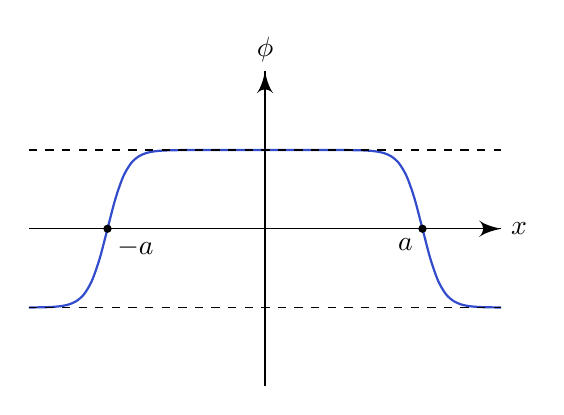
\begin{tikzpicture}
    \draw [->] (-3, 0) -- (3, 0) node [right] {$x$};
    \draw [->] (0, -2) -- (0, 2) node [above] {$\phi$};

    \draw [mblue, thick] plot [smooth] coordinates {(-3.0,-0.99933) (-2.9,-0.99851) (-2.8,-0.99668) (-2.7,-0.99263) (-2.6,-0.98367) (-2.5,-0.96403) (-2.4,-0.92167) (-2.3,-0.83365) (-2.2,-0.66404) (-2.1,-0.37995) (-2.0,-0.00000) (-1.9,0.37995) (-1.8,0.66404) (-1.7,0.83365) (-1.6,0.92167) (-1.5,0.96403) (-1.4,0.98367) (-1.3,0.99263) (-1.2,0.99668) (-1.1,0.99851) (-1.0,0.99933) (-0.9,0.99970) (-0.8,0.99986) (-0.7,0.99994) (-0.6,0.99997) (-0.5,0.99999) (-0.4,0.99999) (-0.3,1.00000) (-0.2,1.00000) (-0.1,1.00000) (0.0,1.00000) (0.1,1.00000) (0.2,1.00000) (0.3,1.00000) (0.4,0.99999) (0.5,0.99999) (0.6,0.99997) (0.7,0.99994) (0.8,0.99986) (0.9,0.99970) (1.0,0.99933) (1.1,0.99851) (1.2,0.99668) (1.3,0.99263) (1.4,0.98367) (1.5,0.96403) (1.6,0.92167) (1.7,0.83365) (1.8,0.66404) (1.9,0.37995) (2.0,-0.00000) (2.1,-0.37995) (2.2,-0.66404) (2.3,-0.83365) (2.4,-0.92167) (2.5,-0.96403) (2.6,-0.98367) (2.7,-0.99263) (2.8,-0.99668) (2.9,-0.99851) (3.0,-0.99933)};
    % map (\x -> (showFFloat (Just 1) x "", showFFloat (Just 5) (tanh (4 * (x + 2)) - tanh (4 * (x - 2)) - 1) "")) [-3,-2.9..3]

    \draw [dashed] (-3, 1) -- (3, 1);
    \draw [dashed] (-3, -1) -- (3, -1);

    \node [circ] at (-2, 0) {};
    \node [anchor = north west] at (-2, 0) {$-a$};

    \node [circ] at (2, 0) {};
    \node [anchor = north east] at (2, 0) {$a$};
  \end{tikzpicture}
\end{center}

Here we have to make the crucial assumption that our kinks are well-separated. Matters get a lot worse when they get close to each other, and it is difficult to learn anything about them analytically. However, by making appropriate approximations, we can understand well-separated kink-antikink configurations.

When the kink and anti-kink are far away, we can separate out the kink and anti-kink. To do so, we first pick a point $b$ lying in between the kink and the anti-kink:

\begin{center}
  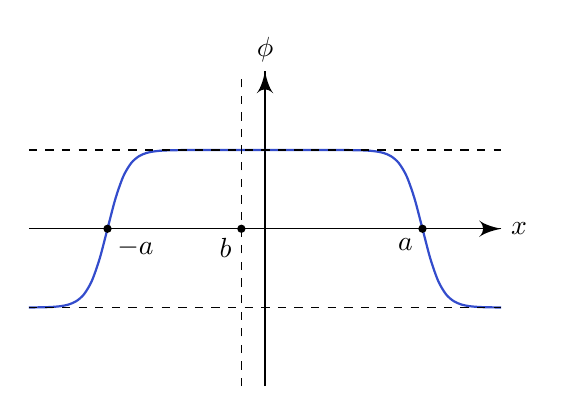
\begin{tikzpicture}
    \draw [->] (-3, 0) -- (3, 0) node [right] {$x$};
    \draw [->] (0, -2) -- (0, 2) node [above] {$\phi$};

    \draw [mblue, thick] plot [smooth] coordinates {(-3.0,-0.99933) (-2.9,-0.99851) (-2.8,-0.99668) (-2.7,-0.99263) (-2.6,-0.98367) (-2.5,-0.96403) (-2.4,-0.92167) (-2.3,-0.83365) (-2.2,-0.66404) (-2.1,-0.37995) (-2.0,-0.00000) (-1.9,0.37995) (-1.8,0.66404) (-1.7,0.83365) (-1.6,0.92167) (-1.5,0.96403) (-1.4,0.98367) (-1.3,0.99263) (-1.2,0.99668) (-1.1,0.99851) (-1.0,0.99933) (-0.9,0.99970) (-0.8,0.99986) (-0.7,0.99994) (-0.6,0.99997) (-0.5,0.99999) (-0.4,0.99999) (-0.3,1.00000) (-0.2,1.00000) (-0.1,1.00000) (0.0,1.00000) (0.1,1.00000) (0.2,1.00000) (0.3,1.00000) (0.4,0.99999) (0.5,0.99999) (0.6,0.99997) (0.7,0.99994) (0.8,0.99986) (0.9,0.99970) (1.0,0.99933) (1.1,0.99851) (1.2,0.99668) (1.3,0.99263) (1.4,0.98367) (1.5,0.96403) (1.6,0.92167) (1.7,0.83365) (1.8,0.66404) (1.9,0.37995) (2.0,-0.00000) (2.1,-0.37995) (2.2,-0.66404) (2.3,-0.83365) (2.4,-0.92167) (2.5,-0.96403) (2.6,-0.98367) (2.7,-0.99263) (2.8,-0.99668) (2.9,-0.99851) (3.0,-0.99933)};

    \draw [dashed] (-3, 1) -- (3, 1);
    \draw [dashed] (-3, -1) -- (3, -1);

    \node [circ] at (-2, 0) {};
    \node [anchor = north west] at (-2, 0) {$-a$};

    \node [circ] at (2, 0) {};
    \node [anchor = north east] at (2, 0) {$a$};

    \draw [dashed] (-0.3, -2) -- (-0.3, 2);
    \node [circ] at (-0.3, 0) {};
    \node [anchor = north east] at (-0.3, 0) {$b$};
  \end{tikzpicture}
\end{center}

The choice of $b$ is arbitrary, but we should choose it so that it is far away from both kinks. We will later see that, at least to first order, the result of our computations does not depend on which $b$ we choose. We will declare that the parts to the left of $b$ belongs to the kink, and the parts to the right of $b$ belong to the anti-kink. Then by integrating the energy-momentum tensor in these two regions, we can obtain the momentum of the kink and the anti-kink separately.

We will focus on the kink only. Its momentum is given by
\[
  P = - \int_{-\infty}^b T^0_1 \;\d x = - \int_{-\infty}^b \dot{\phi} \phi' \;\d x.
\]
Since $T^\mu_\nu$ is conserved, we know $\partial_\mu T^\mu\!_\nu = 0$. So we find
\[
  \frac{\partial}{\partial t} T^0\!_1 + \frac{\partial}{\partial x}T^1\!_1 = 0.
\]
By Newton's second law, the force on the kink is given by the rate of change of the momentum:
\begin{align*}
  \frac{\d}{\d t} P &= -\int_{-\infty}^b \frac{\partial}{\partial t} T^0\!_1\;\d x \\
  &= \int_{-\infty}^b \frac{\partial}{\partial x} T^1\!_1\;\d x\\
  &= \left.T^1\!_1\right|_b\\
  &= \left(-\frac{1}{2} \dot{\phi}^2 - \frac{1}{2} \phi'^2 + U\right)_b
\end{align*}
Note that there is no contribution at the $-\infty$ end because it is vacuum and $T^1\!_1$ vanishes.

But we want to actually work out what this is. To do so, we need to be more precise about what our initial configuration is. In this theory, we can obtain it just by adding a kink to an anti-kink. The obvious guess is that it should be
\[
  \phi(x) \overset{?}{=} \tanh(x + a) - \tanh(x - a),
\]
but this has the wrong boundary condition. It vanishes on both the left and the right. So we actually want to subtract $1$, and obtain
\[
  \phi(x) = \tanh(x + a) - \tanh(x - a) - 1 \equiv \phi_1 + \phi_2 - 1.
\]
Note that since our equation of motion is not linear, this is in general not a genuine solution! Here, this is approximately a solution, because the kink and anti-kink are well-separated. However, there is no hope that this will be anywhere near a solution when the kink and anti-kink are small!

Before we move on to compute $\dot{\phi}$ and $\phi'$ explicitly and plugging numbers in, we first make some simplifications and approximations. First, we restrict our attention to fields that are initially at rest. So we have $\dot{\phi} = 0$ at $t = 0$. Of course, the force will cause the kinks to move, but we shall, for now, ignore what happens when they start moving.

That gets rid of one term. Next, we notice that we only care about the expression when evaluated at $b$. Here we have $\phi_2 - 1 \approx 0$. So we can try to expand the expression to first order in $\phi_2 - 1$ (and hence $\phi_2'$), and this gives
\[
  F = -\frac{1}{2} \left(\phi_1'^2 + U(\phi_1) - \phi_1' \phi_2' + (\phi_2 - 1) \frac{\d U}{\d \phi}(\phi_1)\right)_b.
\]
We have a zeroth order term $\phi_1'^2 + U(\phi_1)$. We claim that this must vanish. One way to see this is that this term corresponds to the force when there is no anti-kink $\phi_2$. Since the kink does not exert a force on itself, this must vanish!

Analytically, we can deduce this from the Bogomolny equation, which says for any kink solution $\phi$, we have
\[
  \phi' = \frac{\d W}{\d \phi}.
\]
It then follows that
\[
  \frac{1}{2} \phi'^2 = \frac{1}{2} \left(\frac{\d W}{\d \phi}\right)^2 = U(\phi).
\]
Alternatively, we can just computing it directly! In any case, convince yourself that it indeed vanishes in your favorite way, and then move on.

Finally, we note that the field equations tell us
\[
  \frac{\d U}{\d \phi}(\phi_1) = \phi_1''.
\]
So we can write the force as
\[
  F = \big(-\phi_1' \phi_2' + (\phi_2 - 1) \phi_1''\big)_b.
\]
That's about all the simplifications we can make without getting our hands dirty. We might think we should plug in the $\tanh$ terms and compute, but that is \emph{too} dirty. Instead, we use asymptotic expressions of kinks and anti-kinks far from their centers. Using the definition of $\tanh$, we have
\[
  \phi_1 = \tanh(x + a) = \frac{1 - e^{-2(x + a)}}{1 + e^{-2(x + a)}} \approx 1 - 2e^{-2(x + a)}.
\]
This is valid for $x \gg -a$, i.e.\ to the right of the kink. The constant factor of $2$ in from of the exponential is called the \term{amplitude} of the tail. We will later see that the $2$ appearing in the exponent has the interpretation of the mass of the field.

For $\phi_2$, take the approximation that $x \ll a$. Then
\[
  \phi_2 - 1= -\tanh(x - a) - 1 \approx -2 e^{2(x - a)}.
\]
We assume that our $b$ satisfies both of these conditions. These are obviously easy to differentiate once or twice. Doing this, we obtain
\[
  -\phi_1' \phi_2' = (-4e^{-2(x + a)})(-4 e^{2(x - a)}) = 16 e^{-4a}.
\]
Note that this is independent of $x$. In the formula, the $x$ will turn into a $b$, and we saw that the force is independent of $b$. Similarly, the other term is
\[
  (\phi_2 - 1) \phi_1'' = (-2e^{2(x - a)}) (-8 e^{-2(x + a)}) = 16 e^{-4a}.
\]
Therefore we find
\[
  F = 32 e^{-4a},
\]
and as promised, this is independent of the precise position of the cutoff $b$ we chose.

We can write this in a slightly more physical form. Our initial configuration was symmetric around the $y$-axis, but in reality, only the separation matters. We write the separation of the pair as $s = 2a$. Then we have
\[
  F = 32 e^{-2s}.
\]
What is the interpretation of the factor of $2$? Recall that our potential was given by
\[
  U(\phi) = \frac{1}{2}(1 - \phi^2)^2.
\]
We can do perturbation theory around one of the vacuums, say $\phi = 1$. Thus, we set $\phi = 1 + \eta$, and then expanding gives us
\[
  U(\eta) = \frac{1}{2} (-2\eta)^2 = \frac{1}{2}m^2 \eta^2,
\]
where $m = 2$. This is the same ``2'' that goes into the exponential in the force.

What about the constant factor of $32$? Recall that when we expanded the kink solution, we saw that the amplitude of the tail was $A = 2$. It turns out if we re-did our theory and put back the different possible parameters, we will find that the force is given by
\[
  F = 2 m^2 A^2 e^{-ms}.
\]
This is an interesting and important phenomenon. The mass $m$ was the \emph{perturbative} mass of the field. It is something we obtain by perturbation theory. However, the same mass appears in the force between the solitons, which are non-perturbative phenomenon!

This is perhaps not too surprising. After all, when we tried to understand the soliton interactions, we took the approximation that $\phi_1$ and $\phi_2$ are close to $1$ at $b$. Thus, we are in some sense perturbing around the vacuum $\phi \equiv 1$.

%The perturbative field theory has a meson of mass $2 \hbar$. You might have not noticed this $\hbar$ when doing quantum field theory, because we set $\hbar = 1$. But this makes sense, because in free field theory, we decompose the quantum field into a lot of harmonic oscillators, and the energy of the harmonic oscillator was $\hbar\omega\left(n + \frac{1}{2}\right)$. SO the $\hbar$ should be here.
%
%However, in our soliton, we do \emph{not} have an $\hbar$. That was not a mistake. We have only been working classically.
%
%The soliton has mass $M = \frac{4}{3}$, and this is much larger than the meson mass. Note that one should choose $\hbar$ to be small for perturbation theory to be justified. However, soliton is non-perturbative and has larger mass than the meson).

We can interpret the force between the kink and anti-kink diagrammatically. From the quantum field theory point of view, we can think of this force as being due to meson exchange, and we can try to invent a Feynman diagram calculus that involves solitons. This is a bit controversial, but at least heuristically, we can introduce new propagators representing solitons, using double lines, and draw the interaction as
\begin{center}
  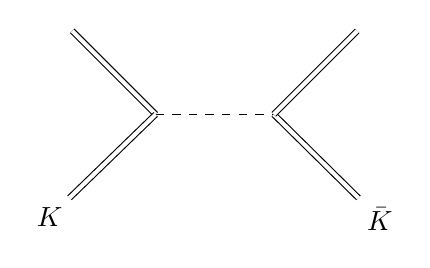
\begin{tikzpicture}
    \begin{feynman}
      \vertex (i);
      \vertex [right=of i] (m);
      \vertex [above right=of m] (f1);
      \vertex [below right=of m] (f2) {$\bar{K}$};
      \vertex [above left=of i] (s1);
      \vertex [below left=of i] (s2) {$K$};

      \diagram*{
        (i) -- [scalar] (m), % label ``meson''
        (f2) -- [double distance=1.5pt] (m) -- [double distance=1.5pt] (f1), % make these double lines
        (s1) -- [double distance=1.5pt] (i) -- [double distance=1.5pt] (s2),
      };
    \end{feynman}
  \end{tikzpicture}
\end{center}
%This is an effective diagram leading to a Yukawa force in $1 + 1$ dimensions, which decays exponentially with separation $s$.
%
%The amplitude of the tail of the of the soliton kink is $A = 2$. The factor of $32$ in the force ultimately comes from the mass being $m = 2$. More generally, one can show that if we put in parameters into our theory, we have
%\[
% F = 2 m^2 A^2 e^{-ms}.
%\]

So what happens to this soliton? The force we derived was positive. So the kink is made to move to the right. By symmetry, we will expect the anti-kink to move towards the left. They will collide!

What happens when they collide? All our analysis so far assumed the kinks were well-separated, so everything breaks down. We can only understand this phenomena numerically. After doing some numerical simulations, we see that there are two regimes:
\begin{itemize}
  \item If the kinks are moving slowly, then they will annihilate into \emph{meson radiation}.
  \item If the kinks are moving very quickly, then bounce off each other.
\end{itemize}
%We can now study the time-dependence. The kinks will accelerate due to standard Newtonian dynamics, and they will move towards each other. However, the full dynamics of the kink-antikink pair is complicated. When they hit each other, they annihilate, and this happens in the regime where the separation is large. Where does the energy go when they annihilate? The answer is that they annihilate into meson radiation, which we can discover by doing numerical simulations.
%
%Annihilation is what happens if they are initially at rest, or slowly moving. However, at high speed, they happen to bounce of each other (of course, there is still some energy loss to radiation). These are very complicated, and we understand this mostly through numerical simulations.

\subsection{Quantization of kink motion}
We now briefly talk about how to quantize kinks. The most naive way of doing so is pretty straightforward. We use the moduli space approximation, and then we have a very simple kink Lagrangian.
\[
  L = \frac{1}{2} M \dot{a}^2.
\]
This is just a free particle moving in $\R$ with mass $M$. This $a$ is known as the \term{collective coordinate} of the kink. Quantizing a free particle is very straightforward. It is just IB Quantum Mechanics. For completeness, we will briefly outline this procedure.

We first put the system in Hamiltonian form. The conjugate momentum to $a$ is given by
\[
  P = M \dot{a}.
\]
Then the Hamiltonian is given by
\[
  H = P \dot{a} - L = \frac{1}{2M} P^2.
\]
Then to quantize, we replace $P$ by the operator $-i\hbar \frac{\partial}{\partial a}$. In this case, the quantum Hamiltonian is given by
\[
  H = - \frac{\hbar^2}{2M} \frac{\partial^2}{\partial a^2}.
\]
A wavefunction is a function of $a$ and $t$, and this is just ordinary QM for a single particle.

As usual, the stationary states are given by
\[
  \psi(a) = e^{i\kappa a},
\]
and the momentum and energy (eigenvalues) are
\[
  P = \hbar \kappa,\quad H = E = \frac{\hbar^2 \kappa^2}{2M} = \frac{P^2}{2M}.
\]

Is this actually ``correct''? Morally speaking, we really should quantize the complete $1 + 1$ dimensional field theory. What would this look like?

In normal quantum field theory, we consider perturbations around a vacuum solution, say $\phi \equiv 1$, and we obtain mesons. Here if we want to quantize the kink solution, we should consider field oscillations around the kink. Then the solution contains both a kink and a meson. These mesons give rise to quantum corrections to the kink mass $M$.

Should we be worried about these quantum corrections? Unsurprisingly, it turns out these quantum corrections are of the order of the meson mass. So we should not be worried when the meson mass is small.

Meson-Kink scattering can also be studied in the full quantum theory. To first approximation, since the kink is heavy, mesons are reflected or transmitted with some probabilities, while the momentum of the kink is unchanged. But when we work to higher orders, then of course the kink will move as a result. This is all very-complicated.

For more details, see Rajaraman's \emph{Solitons and Instantons}, or Weinberg's \emph{Classical Solutions in Quantum Field Theory}.

The thing that is really hard to understand in the quantum field theory is kink-antikink pair production. This happens when the mesons are very fast, and the theory is highly relativistic. What we have done so far is perturbative and makes the non-relativistic approximation to get the adiabatic picture. It is \emph{very} difficult to understand this.

\subsection{Sine-Gordon kinks}
We end the section by briefly talking about kinks in a different theory, namely the \term{sine-Gordon theory}. In this theory, kinks are often known as \term{soltions} instead.

The sine-Gordon theory is given by the potential
\[
  U(\phi) = 1 - \sin \phi.
\]
Again, we suppress coupling constants, but it is possible to add them back.

The potential looks like
\begin{center}
  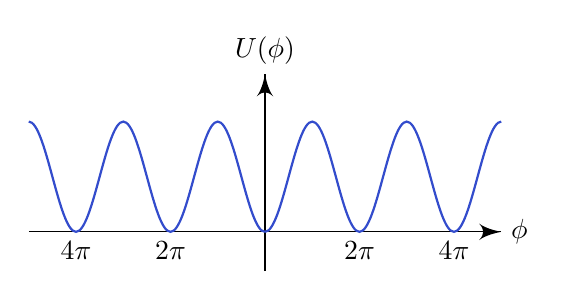
\begin{tikzpicture}
    \draw [->](-3, 0) -- (3, 0) node [right] {$\phi$};
    \draw [->] (0, -0.5) -- (0, 2) node [above] {$U(\phi)$};

    \draw [mblue, thick] (0, 0) cos (0.3, 0.7) sin (0.6, 1.4) cos (0.9, 0.7) sin (1.2, 0) cos (1.5, 0.7) sin (1.8, 1.4) cos (2.1, 0.7) sin (2.4, 0) cos (2.7, 0.7) sin (3, 1.4);;
    \draw [mblue, thick, xscale=-1] (0, 0) cos (0.3, 0.7) sin (0.6, 1.4) cos (0.9, 0.7) sin (1.2, 0) cos (1.5, 0.7) sin (1.8, 1.4) cos (2.1, 0.7) sin (2.4, 0) cos (2.7, 0.7) sin (3, 1.4);;

    \node at (1.2, 0) [below] {$2\pi$};
    \node at (2.4, 0) [below] {$4\pi$};
    \node at (-1.2, 0) [below] {$2\pi$};
    \node at (-2.4, 0) [below] {$4\pi$};
  \end{tikzpicture}
\end{center}
Now there are \emph{infinitely many} distinct vacua. In this case, we find we need to pick $W$ such that
\[
  \frac{\d W}{\d \phi} = 2 \sin \frac{1}{2}\phi. % this is dW/dphi instead
\]

\subsubsection*{Static sine-Gordon kinks}
To find the static kinks in the sine-Gordon theory, we again look at the Bogomolny equation. We have to solve
\[
  \frac{\d \phi}{\d x} = 2 \sin \frac{1}{2}\phi.
\]
This can be solved. This involves integrating a $\csc$, and ultimately gives us a solution of
\[
  \phi(x) = 4 \tan^{-1} e^{x - a}.
\]
We can check that this solution interpolates between $0$ and $2\pi$.

\begin{center}
  \begin{tikzpicture}
    \draw [->] (-4, 0) -- (4, 0) node [right] {$x$};
    \draw [->] (0, -0.5) -- (0, 2.5) node [above] {$\phi$};

    \draw [mblue, thick] plot [smooth] coordinates {(-4.0,0.00000) (-3.9,0.00000) (-3.8,0.00000) (-3.7,0.00001) (-3.6,0.00001) (-3.5,0.00001) (-3.4,0.00001) (-3.3,0.00002) (-3.2,0.00002) (-3.1,0.00003) (-3.0,0.00005) (-2.9,0.00006) (-2.8,0.00008) (-2.7,0.00011) (-2.6,0.00015) (-2.5,0.00020) (-2.4,0.00027) (-2.3,0.00037) (-2.2,0.00050) (-2.1,0.00068) (-2.0,0.00091) (-1.9,0.00123) (-1.8,0.00166) (-1.7,0.00224) (-1.6,0.00303) (-1.5,0.00409) (-1.4,0.00552) (-1.3,0.00745) (-1.2,0.01005) (-1.1,0.01357) (-1.0,0.01831) (-0.9,0.02472) (-0.8,0.03336) (-0.7,0.04502) (-0.6,0.06074) (-0.5,0.08190) (-0.4,0.11035) (-0.3,0.14847) (-0.2,0.19922) (-0.1,0.26607) (0.0,0.35251) (0.1,0.46091) (0.2,0.59053) (0.3,0.73548) (0.4,0.88474) (0.5,1.02559) (0.6,1.14850) (0.7,1.24946) (0.8,1.32902) (0.9,1.39011) (1.0,1.43628) (1.1,1.47087) (1.2,1.49666) (1.3,1.51583) (1.4,1.53006) (1.5,1.54061) (1.6,1.54843) (1.7,1.55423) (1.8,1.55852) (1.9,1.56170) (2.0,1.56406) (2.1,1.56580) (2.2,1.56710) (2.3,1.56806) (2.4,1.56877) (2.5,1.56929) (2.6,1.56968) (2.7,1.56997) (2.8,1.57019) (2.9,1.57034) (3.0,1.57046) (3.1,1.57055) (3.2,1.57061) (3.3,1.57066) (3.4,1.57070) (3.5,1.57072) (3.6,1.57074) (3.7,1.57076) (3.8,1.57077) (3.9,1.57077) (4.0,1.57078)};
    % map (\x -> (showFFloat (Just 1) x "", showFFloat (Just 5) (atan ( exp (3*x - 1))) "")) [-4,-3.9..4]

    \draw [dashed] (-4, 1.57078) -- (4, 1.57078);

    \node [left] at (-4, 0) {$0$};
    \node [right] at (4, 1.57078) {$2\pi$};
    \node [circ] at (0.33, 0.785398) {};
    \draw [dashed] (0.33, 0.785398) -- (0.33, 0) node [below] {$a$};
  \end{tikzpicture}
\end{center}

Unlike the $\phi^4$ theory, dynamical multi-kink solutions can be derived \emph{exactly}. Ultimately, this is due to the sine-Gordon equation being \emph{integrable}. For more details, refer to the IID Integrable Systems course. There are multiple ways to obtain these multi-soliton solutions, such as via the B\"acklund transforms, but we will not go into these. Instead, let's just do some examples.

Dynamical multi-kink solutions can be derived exactly. One of the earlier ways to do so was via B\"acklund transforms, but that was very complicated. People later invented better methods, but they are still not very straightforward.

\begin{eg}
  There is a two-kink solution
  \[
    \phi (x, t) = 4 \tan^{-1} \left(\frac{v \sinh \gamma x}{ \cosh \gamma vt}\right),
  \]
  where, as usual, we have
  \[
    \gamma = (1 - v^2)^{-1/2}.
  \]
  For $v = 0.01$, this looks like
  \begin{center}
    \begin{tikzpicture}
      \draw [->] (-4, 0) -- (4, 0) node [right] {$x$};
      \draw [->] (0, -2.5) -- (0, 2.5) node [above] {$\phi$};

      \draw [mblue, thick] plot [smooth] coordinates {(-4.0,-1.56957) (-3.9,-1.56914) (-3.8,-1.56856) (-3.7,-1.56778) (-3.6,-1.56672) (-3.5,-1.56529) (-3.4,-1.56337) (-3.3,-1.56077) (-3.2,-1.55726) (-3.1,-1.55252) (-3.0,-1.54613) (-2.9,-1.53751) (-2.8,-1.52587) (-2.7,-1.51019) (-2.6,-1.48906) (-2.5,-1.46067) (-2.4,-1.42263) (-2.3,-1.37197) (-2.2,-1.30524) (-2.1,-1.21893) (-2.0,-1.11067) (-1.9,-0.98117) (-1.8,-0.83628) (-1.7,-0.68699) (-1.6,-0.54603) (-1.5,-0.42296) (-1.4,-0.32183) (-1.3,-0.24211) (-1.2,-0.18089) (-1.1,-0.13458) (-1.0,-0.09986) (-0.9,-0.07394) (-0.8,-0.05461) (-0.7,-0.04020) (-0.6,-0.02942) (-0.5,-0.02129) (-0.4,-0.01509) (-0.3,-0.01027) (-0.2,-0.00637) (-0.1,-0.00305) (0.0,0.00000) (0.1,0.00305) (0.2,0.00637) (0.3,0.01027) (0.4,0.01509) (0.5,0.02129) (0.6,0.02942) (0.7,0.04020) (0.8,0.05461) (0.9,0.07394) (1.0,0.09986) (1.1,0.13458) (1.2,0.18089) (1.3,0.24211) (1.4,0.32183) (1.5,0.42296) (1.6,0.54603) (1.7,0.68699) (1.8,0.83628) (1.9,0.98117) (2.0,1.11067) (2.1,1.21893) (2.2,1.30524) (2.3,1.37197) (2.4,1.42263) (2.5,1.46067) (2.6,1.48906) (2.7,1.51019) (2.8,1.52587) (2.9,1.53751) (3.0,1.54613) (3.1,1.55252) (3.2,1.55726) (3.3,1.56077) (3.4,1.56337) (3.5,1.56529) (3.6,1.56672) (3.7,1.56778) (3.8,1.56856) (3.9,1.56914) (4.0,1.56957)};
      \draw [mred, thick] plot [smooth] coordinates {(-4.0,-1.53726) (-3.9,-1.52555) (-3.8,-1.50975) (-3.7,-1.48847) (-3.6,-1.45988) (-3.5,-1.42157) (-3.4,-1.37057) (-3.3,-1.30340) (-3.2,-1.21659) (-3.1,-1.10779) (-3.0,-0.97784) (-2.9,-0.83269) (-2.8,-0.68347) (-2.7,-0.54286) (-2.6,-0.42031) (-2.5,-0.31974) (-2.4,-0.24053) (-2.3,-0.17975) (-2.2,-0.13381) (-2.1,-0.09939) (-2.0,-0.07374) (-1.9,-0.05467) (-1.8,-0.04052) (-1.7,-0.03002) (-1.6,-0.02224) (-1.5,-0.01648) (-1.4,-0.01221) (-1.3,-0.00904) (-1.2,-0.00670) (-1.1,-0.00496) (-1.0,-0.00367) (-0.9,-0.00271) (-0.8,-0.00200) (-0.7,-0.00147) (-0.6,-0.00108) (-0.5,-0.00078) (-0.4,-0.00055) (-0.3,-0.00038) (-0.2,-0.00023) (-0.1,-0.00011) (0.0,0.00000) (0.1,0.00011) (0.2,0.00023) (0.3,0.00038) (0.4,0.00055) (0.5,0.00078) (0.6,0.00108) (0.7,0.00147) (0.8,0.00200) (0.9,0.00271) (1.0,0.00367) (1.1,0.00496) (1.2,0.00670) (1.3,0.00904) (1.4,0.01221) (1.5,0.01648) (1.6,0.02224) (1.7,0.03002) (1.8,0.04052) (1.9,0.05467) (2.0,0.07374) (2.1,0.09939) (2.2,0.13381) (2.3,0.17975) (2.4,0.24053) (2.5,0.31974) (2.6,0.42031) (2.7,0.54286) (2.8,0.68347) (2.9,0.83269) (3.0,0.97784) (3.1,1.10779) (3.2,1.21659) (3.3,1.30340) (3.4,1.37057) (3.5,1.42157) (3.6,1.45988) (3.7,1.48847) (3.8,1.50975) (3.9,1.52555) (4.0,1.53726)};
      % let v = 0.01 in let g = sqrt (1 / (1 - v * v)) in let t = 400 in map (\x -> (showFFloat (Just 1) x "", showFFloat (Just 5) (atan (v * sinh (g * x * 3) / cosh (v * g * t))) "")) [-4,-3.9..4]

      \draw [dashed] (-4, 1.57078) -- (4, 1.57078);
      \draw [dashed] (-4, -1.57078) -- (4, -1.57078);

      \node [right] at (4, 1.57078) {$2\pi$};
      \node [left] at (-4, -1.57078) {$-2\pi$};

      \node [mblue, left] at (1.73, 0.785) {\small$t = 0$};
      \node [mred, right] at (2.85, 0.785) {\small$t = 400$};
    \end{tikzpicture}
  \end{center}

  Note that since $\phi(x, t) = \phi(x, -t)$, we see that this solution involves two solitons at first approaching each other, and then later bouncing off. Thus, the two kinks \emph{repel} each other. This is not too surprising, because when we did kinks in $\phi^4$ theory, we saw that a kink and an anti-kink repelled.

  We can again compute the force just like the $\phi^4$ theory, but alternatively, since we have a full, exact solution, we can work it out directly from the solution! The answers, fortunately, agree. If we do the computations, we find that the point of closest approach is $\sim 2 \log \left(\frac{2}{v}\right)$ if $v$ is small.
\end{eg}

There are some important comments to make. In the sine-Gordon theory, we can have very complicated interactions between kinks and anti-kinks, and these can connect vastly different vacua. However, \emph{static} solutions must join $2n\pi$ and $2(n \pm 1)\pi$ for some $n$, because if we want to join vacua further apart, we will have more than one kink, and they necessarily interact.

If we have multiple kinks and anti-kinks, then teach of these things can have their own velocity, and we might expect some very complicated interaction between them, such as annihilation and pair production. But remarkably, the interactions are \emph{not} complicated. If we try to do numerical simulations, or use the exact solutions we find, we see that we do not have energy loss due to ``radiation''. Instead, the solitons remain very well-structured solitons. This, again, is due to the theory being integrable.

\subsubsection*{Topology of the sine-Gordon equation}
There are also a lot of interesting things we can talk about without going into details about what the solutions look like.

The important realization is that our potential is periodic in $\phi$. For the sine-Gordon theory, it is much better to think of this as a field modulo $2\pi$, i.e.\ as a function
\[
  \phi: \R \to S^1.
\]
In this language, the boundary condition is that $\phi(x) = 0 \bmod 2\pi$ as $x \to \pm \infty$. Thus, instead of thinking of the kink as joining two vacua, we can think of it as ``winding around the circle'' instead.

We can go further. Since the boundary conditions of $\phi$ are the same on two sides, we can join the ends of the domain together, and we can think of $\phi$ as a map
\[
  \phi: S^1 \to S^1
\]
instead. This is a \term{compactification} of the space.

Topologically, such maps are classified by their \term{winding number}, or the \term{degree}, which we denote \term{$Q$}. This is a topological (homotopy) invariant of a map, and is preserved under continuous deformations of the field. Thus, it is preserved under time evolution of the field.

Intuitively, the winding number is just how many times we go around the circle. There are multiple (equivalent) ways of making this precise.

\separator

The first way, which is the naive way, is purely topological. We simply have to go back to the first picture, where we regard $\phi$ as a real value. Suppose the boundary values are
\[
  \phi(-\infty) = 2 n_L \pi,\quad \phi(\infty) = 2 n_R \pi.
\]
Then we set the winding number to be $Q = n_R - n_L$.

Topologically, we are using the fact that $\R$ is the \term{universal covering space}\index{covering space} of the circle, and thus we are really looking at the induced map on the fundamental group of the circle.

\begin{eg}
  As we saw, a single kink has $Q = 1$.
  \begin{center}
    \begin{tikzpicture}
      \draw [->] (-4, 0) -- (4, 0) node [right] {$x$};
      \draw [->] (0, -0.5) -- (0, 2.5) node [above] {$\phi$};

      \draw [mblue, thick] plot [smooth] coordinates {(-4.0,0.00000) (-3.9,0.00000) (-3.8,0.00000) (-3.7,0.00001) (-3.6,0.00001) (-3.5,0.00001) (-3.4,0.00001) (-3.3,0.00002) (-3.2,0.00002) (-3.1,0.00003) (-3.0,0.00005) (-2.9,0.00006) (-2.8,0.00008) (-2.7,0.00011) (-2.6,0.00015) (-2.5,0.00020) (-2.4,0.00027) (-2.3,0.00037) (-2.2,0.00050) (-2.1,0.00068) (-2.0,0.00091) (-1.9,0.00123) (-1.8,0.00166) (-1.7,0.00224) (-1.6,0.00303) (-1.5,0.00409) (-1.4,0.00552) (-1.3,0.00745) (-1.2,0.01005) (-1.1,0.01357) (-1.0,0.01831) (-0.9,0.02472) (-0.8,0.03336) (-0.7,0.04502) (-0.6,0.06074) (-0.5,0.08190) (-0.4,0.11035) (-0.3,0.14847) (-0.2,0.19922) (-0.1,0.26607) (0.0,0.35251) (0.1,0.46091) (0.2,0.59053) (0.3,0.73548) (0.4,0.88474) (0.5,1.02559) (0.6,1.14850) (0.7,1.24946) (0.8,1.32902) (0.9,1.39011) (1.0,1.43628) (1.1,1.47087) (1.2,1.49666) (1.3,1.51583) (1.4,1.53006) (1.5,1.54061) (1.6,1.54843) (1.7,1.55423) (1.8,1.55852) (1.9,1.56170) (2.0,1.56406) (2.1,1.56580) (2.2,1.56710) (2.3,1.56806) (2.4,1.56877) (2.5,1.56929) (2.6,1.56968) (2.7,1.56997) (2.8,1.57019) (2.9,1.57034) (3.0,1.57046) (3.1,1.57055) (3.2,1.57061) (3.3,1.57066) (3.4,1.57070) (3.5,1.57072) (3.6,1.57074) (3.7,1.57076) (3.8,1.57077) (3.9,1.57077) (4.0,1.57078)};
    % map (\x -> (showFFloat (Just 1) x "", showFFloat (Just 5) (atan ( exp (3*x - 1))) "")) [-4,-3.9..4]

      \draw [dashed] (-4, 1.57078) -- (4, 1.57078);

      \node [left] at (-4, 0) {$0$};
      \node [right] at (4, 1.57078) {$2\pi$};
    \end{tikzpicture}
  \end{center}
\end{eg}

Thus, we can think of the $Q$ as the \emph{net soliton number}.

\separator

But this construction we presented is rather specific to maps from $S^1$ to $S^1$. We want something more general that can be used for more complicated systems. We can do this in a more ``physics'' way. We note that there is a \emph{topological} current
\[
  j^\mu = \frac{1}{2\pi} \varepsilon^{\mu\nu} \partial_\nu \phi,
\]
where $\varepsilon^{\mu\nu}$ is the anti-symmetric tensor in $1 + 1$ dimensions, chosen so that $\varepsilon^{01} = 1$.

In components, this is just
\[
  j^\mu = \frac{1}{2\pi} (\partial_x \phi, - \partial_t \phi).
\]
This is conserved because of the symmetry of mixed partial derivatives, so that
\[
  \partial_\mu j^\mu = \frac{1}{2\pi} \varepsilon^{\mu\nu} \partial_\mu \partial_\nu \phi = 0.
\]
As usual, a current induces a conserved charge
\[
  Q = \int j^0 \;\d x = \frac{1}{2\pi} \int \partial_x \phi \;\d x = \frac{1}{2\pi} (\phi(\infty) - \phi(-\infty)) = n_R - n_L,
\]
which is the formula we had earlier.

Note that all these properties do not depend on $\phi$ satisfying any field equations! It is completely topological.

\separator

Finally, there is also a differential geometry way of defining this. We note that the target space $S^1$ has a normalized volume form $\omega$ so that
\[
  \int_{S^1} \omega = 1.
\]
For example, we can take
\[
  \omega = \frac{1}{2\pi}\;\d \phi.
\]
Now, given a mapping $\phi: \R \to S^1$, we can pull back the volume form to obtain
\[
  \phi^* \omega = \frac{1}{2\pi} \frac{\d \phi}{\d x} \;\d x.
\]
We can then define the degree of the map to be
\[
  Q = \int \phi^* \omega = \frac{1}{2\pi}\int_{-\infty}^\infty \frac{\d \phi}{\d x}\;\d x.
\]
This is exactly the same as the formula we obtained using the current!

Note that even though the volume form is normalized on $S^1$, the integral when pulled back is not $1$. We can imagine this as saying if we wind around the circle $n$ times, then after pulling back, we would have pulled back $n$ ``copies'' of the volume form, and so the integral will be $n$ times that of the integral on $S^1$.

\separator

We saw that these three definitions gave the same result, and different definitions have different benefits. For example, in the last two formulations, it is not \emph{a priori} clear that the winding number has to be an integer, while this is clear in the first formulation.

\printindex
\end{document}
